\documentclass{article}
\usepackage{amsmath}
\usepackage{xcolor}
\usepackage{gensymb}
\usepackage{ragged2e}
\usepackage{graphicx}
\usepackage{gensymb}
\usepackage{mathtools}
\newcommand{\mydet}[1]{\ensuremath{\begin{vmatrix}#1\end{vmatrix}}}
\providecommand{\brak}[1]{\ensuremath{\left(#1\right)}}
\providecommand{\norm}[1]{\left\lVert#1\right\rVert}
\newcommand{\solution}{\noindent \textbf{Solution: }}
\newcommand{\myvec}[1]{\ensuremath{\begin{pmatrix}#1\end{pmatrix}}}
\let\vec\mathbf
\begin{document}
\begin{center}
        \textbf\large{CHAPTER-9 \\ AREAS OF PARALLELOGRAMS AND TRIANGLES}
\end{center}
\section{Exercise 9.2}
Q1. In the figure given below, $ABCD$ is a parallelogram, $AE \perp DC$ and $CF \perp AD$.If $AB = 16cm$, $AE = 8cm$ and $CF = 10cm$, find $AD$.\\
\textbf{Construction}
\begin{figure}[H]
 \begin{center}
  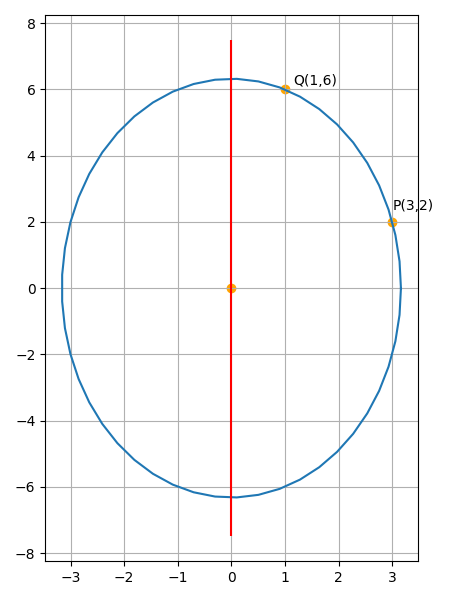
\includegraphics[width=0.75\columnwidth]{fig1.png}
 \end{center}
 \caption{Parallelogram ABCD}
 \label{fig:Fig1}
\end{figure}\\
The following table displays the given input parameters :\\
\begin{table}[H]
	\centering
	%%%%%%%%%%%%%%%%%%%%%%%%%%%%%%%%%%%%%%%%%%%%%%%%%%%%%%%%%%%%%%%%%%%%%%
%%                                                                  %%
%%  This is a LaTeX2e table fragment exported from Gnumeric.        %%
%%                                                                  %%
%%%%%%%%%%%%%%%%%%%%%%%%%%%%%%%%%%%%%%%%%%%%%%%%%%%%%%%%%%%%%%%%%%%%%%

\begin{center}
\begin{tabular}{|c|c|}
\hline
\textbf{Parameter}& \textbf{Value}\\ \hline
$\vec{V}$		 &	$\myvec{0&0\\0&1}$\\ \hline
$\vec{u}$		 &	$\myvec{4\\0}$\\ \hline
$f$				 &  0 \\ \hline
\end{tabular}
\end{center}

	\caption{Input Parameters}
	\label{tab:table1}
\end{table}\\
The lengths and angles which are to be found out are displayed in the table below along with their symbols :\\
\begin{table}[H]
	\centering
	%%%%%%%%%%%%%%%%%%%%%%%%%%%%%%%%%%%%%%%%%%%%%%%%%%%%%%%%%%%%%%%%%%%%%%
%%                                                                  %%
%%  This is the header of a LaTeX2e file exported from Gnumeric.    %%
%%                                                                  %%
%%  This file can be compiled as it stands or included in another   %%
%%  LaTeX document. The table is based on the longtable package so  %%
%%  the longtable options (headers, footers...) can be set in the   %%
%%  preamble section below (see PRAMBLE).                           %%
%%                                                                  %%
%%  To include the file in another, the following two lines must be %%
%%  in the including file:                                          %%
%%        \def\inputGnumericTable{}                                 %%
%%  at the beginning of the file and:                               %%
%%        \input{name-of-this-file.tex}                             %%
%%  where the table is to be placed. Note also that the including   %%
%%  file must use the following packages for the table to be        %%
%%  rendered correctly:                                             %%
%%    \usepackage[latin1]{inputenc}                                 %%
%%    \usepackage{color}                                            %%
%%    \usepackage{array}                                            %%
%%    \usepackage{longtable}                                        %%
%%    \usepackage{calc}                                             %%
%%    \usepackage{multirow}                                         %%
%%    \usepackage{hhline}                                           %%
%%    \usepackage{ifthen}                                           %%
%%  optionally (for landscape tables embedded in another document): %%
%%    \usepackage{lscape}                                           %%
%%                                                                  %%
%%%%%%%%%%%%%%%%%%%%%%%%%%%%%%%%%%%%%%%%%%%%%%%%%%%%%%%%%%%%%%%%%%%%%%



%%  This section checks if we are begin input into another file or  %%
%%  the file will be compiled alone. First use a macro taken from   %%
%%  the TeXbook ex 7.7 (suggestion of Han-Wen Nienhuys).            %%
\def\ifundefined#1{\expandafter\ifx\csname#1\endcsname\relax}


%%  Check for the \def token for inputed files. If it is not        %%
%%  defined, the file will be processed as a standalone and the     %%
%%  preamble will be used.                                          %%
\ifundefined{inputGnumericTable}

%%  We must be able to close or not the document at the end.        %%
 \def\gnumericTableEnd{\end{document}}


%%%%%%%%%%%%%%%%%%%%%%%%%%%%%%%%%%%%%%%%%%%%%%%%%%%%%%%%%%%%%%%%%%%%%%
%%                                                                  %%
%%  This is the PREAMBLE. Change these values to get the right      %%
%%  paper size and other niceties.                                  %%
%%                                                                  %%
%%%%%%%%%%%%%%%%%%%%%%%%%%%%%%%%%%%%%%%%%%%%%%%%%%%%%%%%%%%%%%%%%%%%%%

 \documentclass[12pt%
     %,landscape%
                    ]{report}
       \usepackage[latin1]{inputenc}
       \usepackage{fullpage}
       \usepackage{color}
       \usepackage{array}
       \usepackage{longtable}
       \usepackage{calc}
       \usepackage{multirow}
       \usepackage{hhline}
       \usepackage{ifthen}

 \begin{document}


%%  End of the preamble for the standalone. The next section is for %%
%%  documents which are included into other LaTeX2e files.          %%
\else

%%  We are not a stand alone document. For a regular table, we will %%
%%  have no preamble and only define the closing to mean nothing.   %%
    \def\gnumericTableEnd{}

%%  If we want landscape mode in an embedded document, comment out  %%
%%  the line above and uncomment the two below. The table will      %%
%%  begin on a new page and run in landscape mode.                  %%
%       \def\gnumericTableEnd{\end{landscape}}
%       \begin{landscape}


%%  End of theelse clause for this file being \input.              %%
\fi

%%%%%%%%%%%%%%%%%%%%%%%%%%%%%%%%%%%%%%%%%%%%%%%%%%%%%%%%%%%%%%%%%%%%%%
%%                                                                  %%
%%  The rest is the gnumeric table, except for the closing          %%
%%  statement. Changes below will alter the table's appearance.     %%
%%                                                                  %%
%%%%%%%%%%%%%%%%%%%%%%%%%%%%%%%%%%%%%%%%%%%%%%%%%%%%%%%%%%%%%%%%%%%%%%

\providecommand{\gnumericmathit}[1]{#1} 
%%  Uncomment the next line if you would like your numbers to be in %%
%%  italics if they are italizised in the gnumeric table.           %%
%\renewcommand{\gnumericmathit}[1]{\mathit{#1}}
\providecommand{\gnumericPB}[1]%
{\let\gnumericTemp=\\#1\let\\=\gnumericTemp\hspace{0pt}}
 \ifundefined{gnumericTableWidthDefined}
        \newlength{\gnumericTableWidth}
        \newlength{\gnumericTableWidthComplete}
        \newlength{\gnumericMultiRowLength}
        \global\def\gnumericTableWidthDefined{}
 \fi
%% The following setting protects this code from babel shorthands.  %%
 \ifthenelse{\isundefined{\languageshorthands}}{}{\languageshorthands{english}}
%%  The default table format retains the relative column widths of  %%
%%  gnumeric. They can easily be changed to c, r or l. In that case %%
%%  you may want to comment out the next line and uncomment the one %%
%%  thereafter                                                      %%
\providecommand\gnumbox{\makebox[0pt]}
%%\providecommand\gnumbox[1][]{\makebox}

%% to adjust positions in multirow situations                       %%
\setlength{\bigstrutjot}{\jot}
\setlength{\extrarowheight}{\doublerulesep}

%%  The \setlongtables command keeps column widths the same across  %%
%%  pages. Simply comment out next line for varying column widths.  %%
\setlongtables

\setlength\gnumericTableWidth{%
 53pt+%
 53pt+%
 106pt+%
0pt}
\def\gumericNumCols{3}
\setlength\gnumericTableWidthComplete{\gnumericTableWidth+%
         \tabcolsep*\gumericNumCols*2+\arrayrulewidth*\gumericNumCols}
\ifthenelse{\lengthtest{\gnumericTableWidthComplete > \linewidth}}%
         {\def\gnumericScale{\ratio{\linewidth-%
                        \tabcolsep*\gumericNumCols*2-%
                        \arrayrulewidth*\gumericNumCols}%
{\gnumericTableWidth}}}%
{\def\gnumericScale{1}}

%%%%%%%%%%%%%%%%%%%%%%%%%%%%%%%%%%%%%%%%%%%%%%%%%%%%%%%%%%%%%%%%%%%%%%
%%                                                                  %%
%% The following are the widths of the various columns. We are      %%
%% defining them here because then they are easier to change.       %%
%% Depending on the cell formats we may use them more than once.    %%
%%                                                                  %%
%%%%%%%%%%%%%%%%%%%%%%%%%%%%%%%%%%%%%%%%%%%%%%%%%%%%%%%%%%%%%%%%%%%%%%

\ifthenelse{\isundefined{\gnumericColA}}{\newlength{\gnumericColA}}{}\settowidth{\gnumericColA}{\begin{tabular}{@{}p{53pt*\gnumericScale}@{}}x\end{tabular}}
\ifthenelse{\isundefined{\gnumericColB}}{\newlength{\gnumericColB}}{}\settowidth{\gnumericColB}{\begin{tabular}{@{}p{150pt*\gnumericScale}@{}}x\end{tabular}}
\ifthenelse{\isundefined{\gnumericColC}}{\newlength{\gnumericColC}}{}\settowidth{\gnumericColC}{\begin{tabular}{@{}p{106pt*\gnumericScale}@{}}x\end{tabular}}

\begin{longtable}[c]{%
 b{\gnumericColA}%
 b{\gnumericColB}%
 b{\gnumericColC}%
 }

%%%%%%%%%%%%%%%%%%%%%%%%%%%%%%%%%%%%%%%%%%%%%%%%%%%%%%%%%%%%%%%%%%%%%%
%%  The longtable options. (Caption, headers... see Goosens, p.124) %%
% \caption{The Table Caption.}             \\ %
% \hline % Across the top of the table.
%%  The rest of these options are table rows which are placed on    %%
%%  the first, last or every page. Use \multicolumn if you want.    %%

%%  Header for the first page.                                      %%
% \multicolumn{3}{c}{The First Header} \\ \hline 
% \multicolumn{1}{c}{colTag} %Column 1
% &\multicolumn{1}{c}{colTag} %Column 2
% &\multicolumn{1}{c}{colTag} \\ \hline %Last column
% \endfirsthead

%%  The running header deinition.

%%
% \hline
% \multicolumn{3}{l}{\ldots\small\slshape continued} \\ \hline
% \multicolumn{1}{c}{colTag} %Column 1
% &\multicolumn{1}{c}{colTag} %Column 2
% &\multicolumn{1}{c}{colTag} \\ \hline %Last column
% \endhead

%%  The running footer definition.                                  %%
% \hline
% \multicolumn{3}{r}{\small\slshape continued\ldots} \\
% \endfoot

%%  The ending footer definition.                                   %%
% \multicolumn{3}{c}{That's all folks} \\ \hline 
% \endlastfoot
%%%%%%%%%%%%%%%%%%%%%%%%%%%%%%%%%%%%%%%%%%%%%%%%%%%%%%%%%%%%%%%%%%%%%%

\hhline{|-|-|-}
  \multicolumn{1}{|p{\gnumericColA}|}%
 {\gnumericPB{\raggedright}\gnumbox[l]{Year}}
 &\multicolumn{1}{p{\gnumericColB}|}%
	{\gnumericPB{\raggedright}\gnumbox[l]{Production (in lakh tonnes)}}
 %&\multicolumn{1}{p{\gnumericColC}|}%
 %{\gnumericPB{\raggedright}\gnumbox[l]{Description}}
\\
\hhline{|---|}
  \multicolumn{1}{|p{\gnumericColA}|}%
 {\gnumericPB{\raggedright}\gnumbox[l]{2001}}
 &\multicolumn{1}{p{\gnumericColB}|}%
 {\gnumericPB{\raggedright}\gnumbox[l]{30}}
 %&\multicolumn{1}{p{\gnumericColC}|}%
 %{\gnumericPB{\raggedright}\gnumbox[l]{Vertex A}}
\\
\hhline{|---|}
  \multicolumn{1}{|p{\gnumericColA}|}%
 {\gnumericPB{\raggedright}\gnumbox[l]{2002}}
 &\multicolumn{1}{p{\gnumericColB}|}%
 {\gnumericPB{\raggedright}\gnumbox[l]{35}}
 %&\multicolumn{1}{p{\gnumericColC}|}%
 %{\gnumericPB{\raggedright}\gnumbox[l]{Vertex B}}
\\
\hhline{|---|}
  \multicolumn{1}{|p{\gnumericColA}|}%
 {\gnumericPB{\raggedright}\gnumbox[l]{2003}}
 &\multicolumn{1}{p{\gnumericColB}|}%
 {\gnumericPB{\raggedright}\gnumbox[l]{36}}
 %&\multicolumn{1}{p{\gnumericColC}|}%
 %{\gnumericPB{\raggedright}\gnumbox[l]{Vertex C}}
\\
\hhline{|---|}
  \multicolumn{1}{|p{\gnumericColA}|}%
 {\gnumericPB{\raggedright}\gnumbox[l]{2004}}
 &\multicolumn{1}{p{\gnumericColB}|}%
 {\gnumericPB{\raggedright}\gnumbox[l]{32}}
 %&\multicolumn{1}{p{\gnumericColC}|}%
 %{\gnumericPB{\raggedright}\gnumbox[l]{Midpoint of AC}}
\\
\hhline{|---|}
  \multicolumn{1}{|p{\gnumericColA}|}%
 {\gnumericPB{\raggedright}\gnumbox[l]{2005}}
 &\multicolumn{1}{p{\gnumericColB}|}%
 {\gnumericPB{\raggedright}\gnumbox[l]{37}}
 %&\multicolumn{1}{p{\gnumericColC}|}%
 %{\gnumericPB{\raggedright}\gnumbox[l]{Midpoint of BC}}
\\
\hhline{|---|}
  \multicolumn{1}{|p{\gnumericColA}|}%
 {\gnumericPB{\raggedright}\gnumbox[l]{2006}}
 &\multicolumn{1}{p{\gnumericColB}|}%
 {\gnumericPB{\raggedright}\gnumbox[l]{40}}
 %&\multicolumn{1}{p{\gnumericColC}|}%
 %{\gnumericPB{\raggedright}\gnumbox[l]{Midpoint of AB}}
\\
\hhline{|-|-|-|}
\end{longtable}

\ifthenelse{\isundefined{\languageshorthands}}{}{\languageshorthands{\languagename}}
\gnumericTableEnd

	\caption{Unknown Parameters}
	\label{tab:table2}
\end{table}\\
The input co-ordinates of the above parallelogram is $\vec{D}$ which is at the origin.The rest of the point co-ordinates can be derived based on this assumption in the following way which is shown in the table below :\\
\begin{table}[H]
	\centering
	\begin{tabular}{|c|c|}
\hline
Point & Co-ordinates\\
\hline
$\vec{A}$ & $r\myvec{\cos{\theta}\\\sin{\theta}}$ \\
\hline
$\vec{B}$ & $\vec{A} + \vec{C}$ \\
\hline
$\vec{C}$ & $c\vec{e_1}$\\
\hline
$\vec{E}$ & $d\vec{e_1}$ \\
\hline
$\vec{F}$ & $f\myvec{\cos{\theta}\\\sin{\theta}}$ \\
\hline
\end{tabular}

	\caption{Unknown Co-ordinates}
	\label{tab:table3}
\end{table}\\
\textbf{Deriving the Unknown lengths and angles in terms of known and derived parameters :}\\
\begin{enumerate}
	\item \textbf{Deriving c:}
		From Figure\ref{fig:Fig1}, $c$ is  parallel to $l$(AB paralle to CD).So,
		\begin{align}
			c = l
			\label{eq:1}
		\end{align}
	\item \textbf{Deriving d:}
		From $\triangle{ADE}$,
		\begin{align}
			\cos{\theta} = \frac{DE}{AD} = \frac{d}{r}
			\implies d = r\cos{\theta}
			\label{eq:2}
		\end{align}
	\item \textbf{Deriving r:}
		From $\triangle{ADE}$,
		\begin{align}
			\sin{\theta} = \frac{AE}{AD} = \frac{b}{r}
			\implies r = \frac{b}{\sin{\theta}}
			\label{eq:3}
		\end{align}
	\item \textbf{Deriving f:}
		From $\triangle{DFC}$,
		\begin{align}
			\cos{\theta} = \frac{DF}{DC} = \frac{f}{c}
			\implies f = c\cos{\theta}
			\label{eq:4}
		\end{align}
	\item \textbf{Finding $\theta$:}
		From $\triangle{DFC}$,
		\begin{align}
			\sin{\theta} = \frac{CF}{CD} = \frac{a}{c}
			\implies \theta = \sin^{-1}\frac{a}{c}
			\label{eq:6}
		\end{align}
\end{enumerate}
From eq\ref{eq:1},eq\ref{eq:2},eq\ref{eq:3},eq\ref{eq:4} and eq\ref{eq:6}, table\ref{tab:table2} can be modified as :\\
\begin{table}[H]
	\centering
	\begin{tabular}{|c|c|c|}
\hline
Symbol & value & Description\\
\hline
$c$ & $l$ & DC\\
\hline
$r$ & $\frac{b}{\sin{\theta}}$ & AD \\
\hline
$d$ & $r\cos{\theta}$ & DE \\
\hline
$\theta$ & $\sin^{-1}\frac{a}{c}$ & $\angle{D}$ \\
\hline
$f$ & $c\cos{\theta}$ & DF\\
\hline
\end{tabular}


	\caption{Unknown parameters in terms of known and derived parameters}
	\label{tab:table4}
\end{table}\\
\textbf{Finding out unknown lengths and angles :}\\
\begin{enumerate}
	\item \textbf{Finding $\theta$:}
		From eq\ref{eq:6},
		\begin{align}
			\theta = \sin^{-1}\frac{10}{16} = 38.68\degree
			\label{eq:7}
		\end{align}
	\item \textbf{Finding c:}
		From eq\ref{eq:1},
		\begin{align}
			c = 16cm
			\label{eq:8}
		\end{align}
	\item \textbf{Finding r:}
		From \ref{eq:3}, the value of $r$ is :
		\begin{align}
			r = \frac{8}{\sin{38.68}} = 12.8cm
			\label{eq:9}
		\end{align}
	\item \textbf{Finding d:}
		From eq\ref{eq:2},
		\begin{align}
			d = (12.8)\cos{38.68} = 10cm
			\label{eq:10}
		\end{align}
	\item \textbf{Finding f:}
		From eq\ref{eq:4},
		\begin{align}
			f = (16)\cos{38.68} = 12.48cm
			\label{eq:11}
		\end{align}
\end{enumerate}
\textbf{Deriving co-ordinates in terms of known and derived parameters:}\\
Based on table\ref{tab:table4}, table\ref{tab:table3} can be modified as follows :\\
\begin{table}[H]
	\centering
	\begin{tabular}{|c|c|c|}
\hline
Point & Co-ordinates\\
\hline
$\vec{A}$ & $\frac{b}{\sin{\theta}}\myvec{\cos{\theta}\\\sin{\theta}}$\\
\hline
$\vec{B}$ & $\vec{A} + \vec{C}$\\
\hline
$\vec{C}$ & $c\vec{e_1}$\\
\hline
$\vec{E}$ & $r\cos{\theta}\vec{e_1}$\\
\hline
$\vec{F}$ & $c\cos{\theta}\myvec{\cos{\theta}\\\sin{\theta}}$\\
\hline
\end{tabular}

	\caption{Co-ordinates in terms of known and derived co-ordinates}
	\label{tab:table5}
\end{table}\\
Based on eq\ref{eq:7},eq\ref{eq:8},eq\ref{eq:9},eq\ref{eq:10} and eq\ref{eq:11} and table\ref{tab:table5}.The final co-ordinates of the  parallelogram are displayed in the table below:\\
\begin{table}[H]
	\centering
	\begin{tabular}{|c|c|}
\hline
Point & Co-ordinates\\
\hline
$\vec{A}$ & $\myvec{10\\8}$\\
\hline
$\vec{B}$ & $\myvec{26\\8}$\\
\hline
$\vec{C}$ & $\myvec{16\\0}$\\
\hline
$\vec{D}$ & $\myvec{0\\0}$\\
\hline
$\vec{E}$ & $\myvec{10\\0}$\\
\hline
$\vec{F}$ & $\myvec{9.75\\7.8}$\\
\hline
\end{tabular}

	\caption{Final Co-ordinates}
	\label{tab:table6}
\end{table}\\
From eq\ref{eq:9}, we got the length of AD = r = 12.8cm.
\end{document}
